\documentclass{article}

% Language setting
% Replace `english' with e.g. `spanish' to change the document language
\usepackage[utf8]{inputenc}
\usepackage[T1]{fontenc}
\usepackage[french]{babel}
\usepackage{authblk}        % gestion auteurs/affiliations
% Set page size and margins
% Replace `letterpaper' with `a4paper' for UK/EU standard size
\usepackage[letterpaper,top=2cm,bottom=2cm,left=3cm,right=3cm,marginparwidth=1.75cm]{geometry}

\usepackage[left, modulo]{lineno}
\linenumbers

% Useful packages
\usepackage{tabularx}
\usepackage{array}
\renewcommand{\arraystretch}{1.3}
\usepackage{rotating}
\usepackage{amsmath}
\usepackage{graphicx}
\usepackage[colorlinks=true, allcolors=blue]{hyperref}
\usepackage{csquotes} % très recommandé avec biblatex
\usepackage[backend=biber,style=authoryear]{biblatex} 
\addbibresource{ifall_bordeau.bib} % nom de ton fichier .bib

\title{Lost in Navigation? Ensuring Living Lab Frameworks Stay on Course with Local Needs}
%\title{De l'anthologie de l'absurde à la symphonie locale : trajectoire d'un projet qui a touché terre}
% Auteurs (indices entre crochets = affiliations)
\author[6,5]{E. Delay\thanks{etienne.delay@cirad.fr}}
\author[1]{A.Hertzog-Adamczewski}
\author[3,4]{R. Duboz} % email en note
\author[1,2]{A. Ogilvie}
\author[5]{W. Daré}
\author[6]{A. Bah}
\author[7]{O. Samaké}

% Affiliations
\affil[1]{CIRAD, UMR G-EAU, F-34398 Montpellier, France.}
\affil[2]{IRD, UMR G-EAU, F-34398 Montpellier, France.}
\affil[3]{CIRAD, UMR ASTRE, F-34398 Montpellier, France.}
\affil[4]{IRD, UMI UMMISCO, Hann Mariste, Dakar, Sénégal}
\affil[5]{CIRAD, UMR SENS, F-34398 Montpellier, France.}
\affil[6]{CIRAD, UMR SENS, Ecole Superieur polytechnique de Dakar, UCAD, Sénégal}
\affil[6]{SAED, Saint-Louis, Sénégal}

\begin{document}
\maketitle

\begin{abstract}
Participatory modeling approaches, particularly those rooted in Companion Modeling (ComMod), are often credited with initiating socio-environmental transformations. Examples from Zimbabwe \parencite{perrotton_my_2017} and Burkina Faso \parencite{dare_dynamique_2016} illustrate how these methods have facilitated engagement between stakeholders, sometimes leading to institutional changes over extended periods. However, the effectiveness of such approaches is contingent on their alignment with local realities and pressing challenges. The question remains: who holds the compass in these participatory frameworks? Do researchers, institutions and players succeed in abandoning their agenda? A case study from the Lake Guiers region in Senegal highlights the tensions between knowledge production, local agency, and transformative action.

After several years of engagement with local communities through participatory workshops, a pivotal moment occurred in different arena : when a doctoral student presented her findings on hazardous chemical pollutants in the lake's water, when allochtone populations spoke out against their refusal to respect fishing restrictions face to face with native fishermen (Delay et al. 2023).  Unlike previous discussions on ecosystem management, which were perceived as peripheral to daily survival, this revelation directly impacted livelihoods, exposing communities to immediate and invisible risks. The local response—calls for awareness campaigns and regulatory interventions—raised deeper questions about the adequacy of conventional participatory approaches. How can living lab models move beyond knowledge dissemination towards tangible systemic transformation? How can scientific findings generate experiential urgency rather than passive information?

Recent scholarship suggests that for knowledge to trigger action, it must engage stakeholders not just intellectually/abstract, but affectively — a concept referred to as "affective knowing" \parencite{hertz_knowledge_2025}. This perspective challenges traditional scientific detachment and underscores the need for transformative science that actively catalyzes change rather than merely observing it. A more reflexive and adaptive governance model is necessary—one that situates knowledge within local dispositifs (assemblages of discourses, institutions, and power structures). Rather than assuming that participatory models inherently lead to transformation, they must be reconfigured to align with the strategic urgencies of a given territory. This shift demands a reconsideration of the role of scientists in participatory governance: are they facilitators, guides, or interveners? By embedding participatory models within affective and political landscapes, living labs in Senegal and beyond can become true engines of systemic change rather than passive spaces for stakeholder dialogue.
\end{abstract}

\section{Introduction}

L'avenir est radicalement incertain. Aussi, les acteurs orientent leurs décisions à partir d'imaginaires et de récits appuyés souvent par des technologies calculatoires (modèles, algorithmes, dispositifs de prévision). \textcite{beckert_uncertain_2018} proposent de parler d' "attentes fictionnelles" (plutôt que "rationnelles") : ces fictions, socialement partagées, coordonnent l'action et ont des effets performatifs.

Le projet Santés \& Territoires, a dès son montage souhaité s'inscrire dans une approche intégrant les imaginaires des populations locales et des chercheurs impliqués sur les territoires d'investigation du projet pour essayer de prendre en compte les imaginaires porter par chacune des parties prenantes.  L'objectif du projet Santés \& Territoires\footnote{santes-territoires.org} (2021-2026) est d'accompagner la transition agroécologique dans un cadre \textit{One Health} par la mise en place de \textit{Living Labs}. D'après le \textit{One Health High-Level Expert Panel (OHHLEP)}, le \textit{One Health} est une approche intégrée de la santé qui consiste à équilibrer et à optimiser durablement la santé des personnes, des animaux et des écosystèmes. \textit{One Health} reconnaît que la santé des humains, des animaux domestiques et sauvages, des plantes et de l'environnement en général sont étroitement liées et interdépendantes\footnote{https://www.who.int/groups/one-health-high-level-expert-panel, accessed August, 21, 2025}. En conséquence, le \textit{One Health} est une approche interdisciplinaire et multi-sectorielle. À l'origine, \textit{One Health} est principalement porté par la santé publique vétérinaire et la santé publique pour s'intéresser aux maladies humaines d'origine animale (les zoonoses). Depuis l'adhésion du Programme des Nations Unies pour Environnement (PNUE) en 2022 à l'entente quadripartite formée avec l'Organisation Mondiale de la Santé (OMS), l'Organisation Mondiale de la Santé Animale (OMSA) et l'organisation des Nations Unies pour l'alimentation et l'agriculture (FAO), les applications du concept \textit{One Health} peinent à intégrer les dimensions écologiques et agricoles dans leur actions, alors que ces domaines jouent un rôle central pour la santé des personnes et de l'environnement. Pour contribuer à une meilleure prise en compte de l'écologie et de l'agriculture, le projet Santés \& Territoires opérationnalise l'approche \textit{One Health} en se plaçant dans le cadre de la santé des systèmes socio-écologiques tel que définit par \textcite{de_garine-wichatitsky_health_2021}, et en se basant sur une approche intégrée de la santé, systémique et participative \parencite{duboz_systems_2018}. L'implication de l'ingénieurie participative et des systèmes socio-écologiques permet de bénéficier d'outils, de méthodes et d'un cadre théorique réellement transdisciplianire pour instrumentaliser le dialogue sciences-sociétés.

Pour \textcite{pfotenhauer_learning_2012} on ne peut pas séparer les approches techniques et les approches sociales. Les objets du monde réel sont intimement connecter à la vie des gens qui les utilisent et qui vivent autour. Il est dont nécessaire d'impliquer les population et les politiques dans la prise de décision.

Notre démarche méthodologique s’appuie sur une observation longitudinale du projet Santés \& Territoires au Sénégal, à travers l’analyse de la littérature grise produite par les membres du projet et déposée sur une plateforme de partage, ainsi que sur nos notes de terrain. L’objectif est d’identifier les séquences, ce que \textcite{jasanoff_constitutional_2011} appel “moments constitutionnels”, où l’affect intervient dans l’émergence ou la reconfiguration d’un agencement, c’est-à-dire lorsque les cadres représentationnels habituels ne suffisent plus et que de nouvelles significations — identitaires, mémorielles ou d’appartenance — transforment les relations et recomposent l’agencement \parencite{hertz_knowledge_2025}. Ces moments sont des fenêtres analytiques où les imaginaires dominants sont contestés et réalignés.

Notre ré-interprétation des événements du projet se base sur deux axes conceptuels : \textit{(i)} l'objectif d'émancipation des parties prenantes qui est soutenu par la charte de l'accompagnement définie par le collectif ComMod~\parencite{barreteau_our_2003} poser comme pré-requis de l'action dans le projet, \textit{(i)} \textit{One-health} comme fil rouge du projet qui permet de s'assurer (autant que faire se peut, nous le verrons) d'un alignement de valeur pour les participants du projet. En effet, comme pour \textcite[p.144]{beck_governance_2021} qui étudie la notion de \textit{sustainability}, nous observons derrière la volonté collective de travailler dans un contexte \textit{One Health}, des différences sectorielles persistantes, soutenues par des conflits de valeur ou d'imaginaire et des variations interculturelles dans les pratiques de recherche sont autant d'obstacle à l'alignement des valeurs.

Or il s'agit dans le projet Santés \& territoires d'examiner les liens entre les façons de représenter et de connaître des phénomène d'une part, et les façons d'agir sur eux afin de le transformer, d'autre part. Parce que c'est bien de cela qu'il s'agit ! Accompagner les transformations de pratiques, cultural et culturel en vue d'améliorer la santé globale du socio-éco-système. 

Dans ce papier, nous nous inscrivons donc à la suite de la question de \textcite[p.148]{beck_governance_2021} "\textit{how citizenship gets imagined and enacted; who gets to participate and who is entitled to speak for sustainable futures, as well as who does not belong and hence lacks such voice ?}", en nous intéressant aux reconfigurations opérationnelles a l'\oe{}uvre dans les dynamiques des \textit{Living-Labs} du projet au Sénégal.

%La modélisation d'accompagnement (ComMod) et, plus largement, la modélisation avec parties prenantes, visent un alignement des représentations et des règles d'action par des jeux de rôle, scénarios et modèles co-construits. Cela rouvre le couloir des possibles quand des cadrages experts l'avaient resserré. Dit autrement : si les STI “ferment/ouvrent” des voies, ComMod est une methode et une posture d'alignement délibératif pour ré-articuler imaginaires, controverses et apprentissages collectifs.

%Pour \textcite[p. 82]{pfotenhauer_learning_2012} "Contrairement à notre conception commune de la modélisation, les modèles de systèmes sociotechniques échappent souvent à la validation empirique qui est la pierre angulaire de la qualité technique."


\section{Matériel et méthodes}
\subsection{Cadre théorique : l'approche par les agencements}

Le cadre théorique mobilisé dans cet article s'appuie sur l'approche par les agencements souvent marqué de l'Actor Network theory \parencite{callon_techno-economic_1990, goulet_characterizing_2021} et auxquels \textcite{hertz_knowledge_2025} viennent y ajouter les affectes. Ainsi, un agencement peut être défini comme une configuration dynamique réunissant des éléments hétérogènes, qu'ils soient humains ou non humains, matériels ou immatériels, discursifs ou pratiques. La notion d'agencement recouvre en partie la notion de dispositifs proposés par \textcite{foucault_jeu_1977}. La spécificité des agencements pour \textcite{hertz_knowledge_2025} réside dans sa capacité à générer une expérience commune forte, que les auteurs qualifient d'\textit{affect}, c'est-à-dire une intensité expérientielle capable de déclencher des actions concrètes et situées. Cette approche permet ainsi de dépasser une conception purement représentative ou abstraite de la connaissance pour intégrer pleinement les dimensions sensibles et relationnelles des savoirs produits collectivement.

L'affect renvoie ici à l'idée selon laquelle les connaissances véritablement opérantes ne peuvent pas se limiter à un contenu discursif abstrait : elles doivent être ressenties et vécues pour produire des effets réels sur les acteurs impliqués. L'approche par les agencements souligne ainsi que c'est par la rencontre et l'interaction entre des corps, des pratiques, des discours et des sensibilités que les savoirs acquièrent leur potentiel transformateur \parencite{bessy_experts_1995}. De la même manière ont retrouves dans les travaux de \textcite{jasanoff_constitutional_2011, beck_governance_2021} la notions d'affect dans l'appel des auteurs a convoquer des imaginaires qui pourront faire bouger les fenêtre d’opportunité dans l'innovation.

L'alignement correspond à l'articulation progressive et souvent imprévisible d'éléments initialement dispersés ou en tension. Ce processus nécessite généralement un contexte relationnel favorable, propice à la reconnaissance mutuelle des savoirs mobilisés par des acteurs aux représentations variées \parencite{geels_typology_2007}. \textcite{jasanoff_constitutional_2011, hertz_knowledge_2025} insistent notamment sur l'importance de moments concrets et situés, tels que des activités participatives ou des expériences partagées, qui permettent aux différents éléments de l'agencement de se rapprocher progressivement pour produire un monde en commun \parencite{arendt_condition_1957}.

Enfin, l'approche par les agencements appelle à une posture réflexive renouvelée pour les chercheurs et praticiens impliqués dans des démarches de co-production. Ceux-ci sont invités à devenir des << gestionnaires de sens >> plutôt que de simples producteurs ou transmetteurs de savoir. Leur rôle consiste à faciliter les conditions propices à l'émergence d'affects partagés, susceptibles de fédérer durablement les acteurs autour d'un savoir-action commun. Ce changement de posture implique également de valoriser des méthodes flexibles, ouvertes à l'imprévu et sensibles aux dynamiques affectives qui traversent tout processus collectif de production de connaissances.

\subsection{Evolution chronologie des living-lab du Sénégal}

La première phase, celle du diagnostic, a occupé la première année. Elle a permis de dessiner les cartes des localités et des arènes d’acteurs où viendraient s’ancrer les living-labs, ces lieux d’expérimentation fragiles. Le projet a initié deux Living-Labs autour du lac de Guiers, un dans la commune de Mbane et l'autre dans la commune de Keur Momar Sarr (voir section~\ref{sec:Phaseinit}). 

Dans ces lieux, les chercheurs ont repéré des problématiques qui ne sont pas seulement des << problèmes >> au sens institutionnel, mais des points d’accroche, des lignes de fuite autour desquelles se sont formés des groupes thématiques interdisciplinaires. L’ambition n’était pas de reconduire le poids des cadres institutionnels, mais d'essayer d'inventer avec les habitants des questions qui prennent racine dans le local, qui s’attachent à ce qui persiste, qui fassent sens malgré tout. Cela s’est joué surtout en deuxième année (sec. \ref{sec:phaseIntermediaire}), au moment où les participants de chaque lieu, lentement, ont commencé à entrer dans le processus. Leur intégration dépendait moins de leur disponibilité que de la capacité des animateurs à changer de posture : à renoncer au rôle de pilotes pour se risquer dans le trouble d’un co-accompagnement.

À partir de la troisième année, les activités enracinées dans la matérialité des lieux se sont épaissies. Elles ont commencé à tisser des fils d’interactions imprévues, à faire surgir des synergies que personne n’avait anticipées (sec. \ref{sec:phaseAgencements}). Certaines initiatives, portées par des groupes dispersés, trouvaient soudain des résonances ailleurs : un écho fragile, mais suffisant pour que des mondes se reconnaissent et s’agencent.

Chaque année, les scientifiques se retrouvaient dans une assemblée annuelle -- un moment où les hypothèses s’échangent encore à l’état de germes, où les résultats sont hésitants, en cours de sédimentation.

À partir de la deuxième année, d’autres scènes se sont ouvertes : les Kourel, ces forums organisés dans les villages. Espaces de parole et de négociation, ils ont permis de discuter des activités en cours et de réorienter les enquêtes. Peu à peu, ces Kourel ont pris de l’importance, déplaçant le centre de gravité du pilotage du projet. Dans ces arènes fragiles, où l’incertitude est partagée, se loge aussi un espoir discret : qu’au moment de la clôture du projet, dans deux ans, les participants de ces « événements constitutionnels » soient en mesure d’interpeller directement le monde de la recherche et du développement, en portant la voix des premiers concernés : les habitants.

\subsection{Documentation \textit{in itinere}}
Le projet a réussi à mettre en place une pratique assez peu répandue dans les projets de recherche-actions dans les Suds globaux : la mise en ligne sur une espace de stockage commun des documents hétérogènes produit durant le projet. Après 3 ans de travail au Sénégal, les chercheurs du projet (plus d'une cinquantaine) on produit et mis en commun pas moins de 2437 documents (jpg, pdf, docx...) pour le Sénégal (c.f. fig. \ref{fig:filetype}).

\begin{figure}
    \centering
    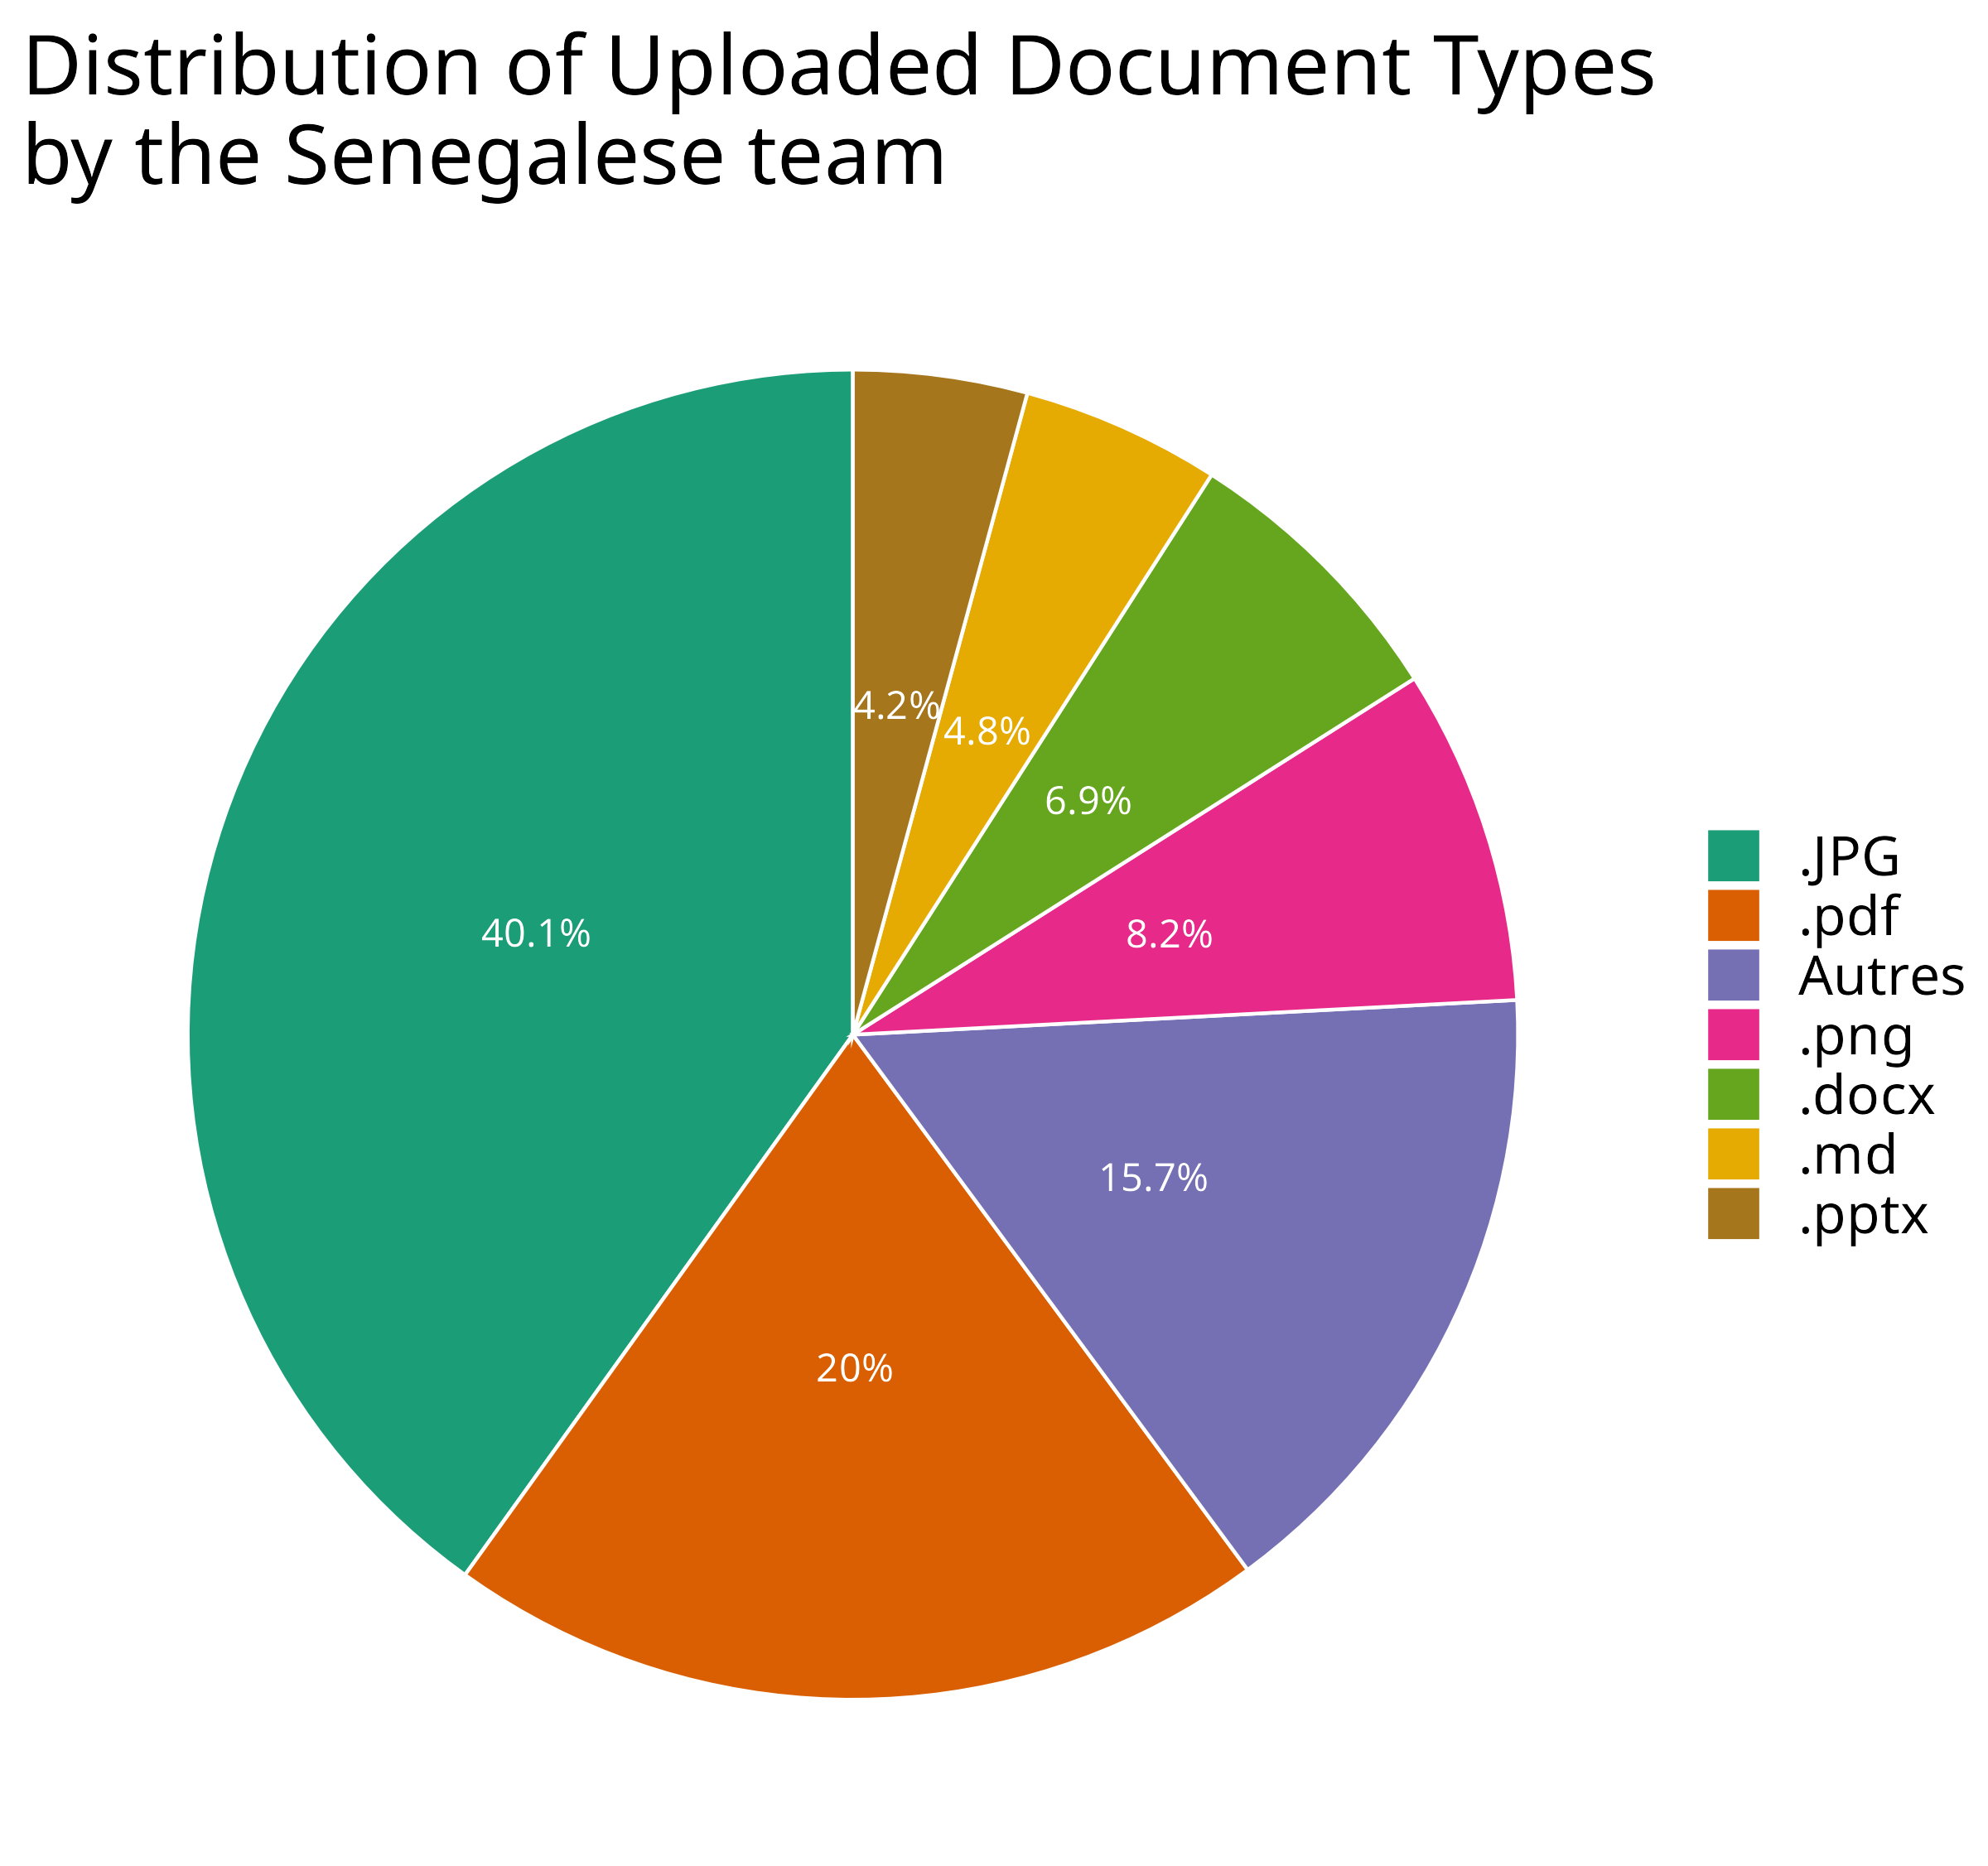
\includegraphics[width=0.6\linewidth]{img/doc_proportion.png}
    \caption{proportion des différents types de documents présents dans le cloud "Sénégal" du projet Santé et territoire. Sur les 9go de données stockés, on dénombre 35 type de documents. Parmi ceux-là, voilà les 7 catégories qui représentent plus de 4\% des données. Les images représente 48\% des documents (jpg+png), et les documents textuels 35\% (pdf+docx+md+pptx)}.
    \label{fig:filetype}
\end{figure}

On peut donc se rendre compte que les données produites par la recherche ne sont que peut présentes, mais que les documents de synthèse eux, sont bien mis en ligne. Dans les travaux que nous avons réalisés, nous nous sommes appuyés sur deux sources différentes : les données textuelles de la plateforme, et nos notes individuelles prises lors des temps fort collectifs. 

Parmi les documents de la plateforme, nous nous sommes appuyés exclusivement sur les sources écrites en donnant un poids plus important aux éléments produits pour les "évenements constitutionel" \textcite{jasanoff_constitutional_2011} que sont les comités scientifiques (constitutif du volet recherche) et les données issues des kourels, dans lesquels les populations locales des LL sont impliquées.

\section{Résultats : les phases de l'alignement}
En traitant ces différentes sources écrites, nous avons identifié trois temps différents : \textit{(i)}, une phase initiale où chaque groupe avance selon sa propre compréhension des enjeux et de son agenda, \textit{(ii)} une phase intermédiaire, ou de nouvelles alliances font jour, certains groupes disparaissent et d'autres se forment, \textit{(iii)} des passerelles commence à exister entre les groupes, ce qui leur permet de conserver leur identité tout en construisant de la synergie avec les autres groupes.

\subsection{Phase initiale : des éléments disjoints}\label{sec:Phaseinit}
Au début du projet, les éléments sont dispersés. Les représentations, intérêts et registres de savoir sont divergents, voire incompatibles. Les dynamiques sont alors marquées par l'inertie ou l'incompréhension mutuelle malgré le fait que les chercheurs affiche des mots clefs communs (tab. \ref{tab:resultcs1}).

\begin{table}[h!]
\centering
\footnotesize
\begin{tabularx}{\textwidth}{>{\raggedright\arraybackslash}p{3.2cm} X X}
\hline
\textbf{Interaction Thématiques} & \textbf{Convergences (alignements)} & \textbf{Divergences (visions distinctes)} \\
\hline
Santé animale / Pastoralisme \& santé animale 
& • Approche participative avec éleveurs, vétérinaires, techniciens. \newline 
• Focus sur surveillance des maladies émergentes et hydriques. \newline
• Importance du lien eau $\leftrightarrow$ santé animale. \newline
• Volonté de renforcer les capacités locales. 
& • Santé animale met l'accent sur multiacteurs et gouvernance territoriale. \newline
• Pastoralisme insiste davantage sur l'accès à l'eau et les maladies hydriques liées au pastoralisme. \\
\hline
Santé humaine / Santé animale 
& • Approche participative du diagnostic. \newline
• Surveillance des maladies émergentes (hydriques + zoonoses). \newline
• Mise en place de protocoles de suivi et systèmes de notification.
& • Santé humaine élargit vers la bio-banque, dépistages et recherche biomédicale. \newline
• Santé animale reste davantage orientée sur la co-construction locale et pratique vétérinaire. \\
\hline
Santé humaine / Biodiversité aquatique 
& • Intérêt partagé pour les maladies hydriques et mollusques vecteurs. \newline
• Détection précoce via protocoles de suivi. \newline
• Vision One-Health commune.
& • Santé humaine vise les maladies émergentes chez l'homme (Fièvre Congo, bilharziose). \newline
• Biodiversité aquatique s'oriente plus sur les biomarqueurs, qualité de l'eau, cyanotoxines. \\
\hline
Biodiversité aquatique / Groupe eau-sol-plante
& • Analyses de qualité de l'eau, impacts des intrants agricoles. \newline
• Mise en place d'un système de monitoring régulier. \newline
• Orientation One-Health / One-Biodiversity.
& • Biodiversité aquatique s'appuie sur une approche écosystémique et halieutique. \newline
• Groupe sol-plante met davantage l'accent sur la fertilité agricole et les flux de biomasse. \\
\hline
Santé sociétale / Santé alimentaire
& • Diagnostic par enquêtes qualitatives et quantitatives. \newline
• Importance des conditions sociales, culturelles et de travail. \newline
• Volonté de renforcer la résilience des acteurs locaux.
& • Santé sociétale : vision centrée sur les déterminants sociaux, empowerment, équité. \newline
• Santé alimentaire : plus focalisée sur systèmes alimentaires, flux, sécurité nutritionnelle. \\
\hline
Santé sociétale / Prospective territoriale
& • Approche participative et prospective avec les acteurs locaux. \newline
• Importance des facteurs sociaux et culturels. \newline
• Volonté de co-construire les scénarios de résilience.
& • Santé sociétale agit sur le court-moyen terme avec indicateurs sociaux. \newline
• Prospective vise une vision long-terme (2040) avec scénarios anticipatifs. \\
\hline
Pesticides / Groupe sol-plante
& • Orientation agro-écologique (réduction des intrants chimiques, alternatives durables). \newline
• Intégration des plantes locales comme biopesticides. \newline
• Intérêt commun pour la formation des producteurs et l'innovation numérique.
& • Pesticides : focalisation sur la réglementation, IA (deep learning) et outils numériques. \newline
• Sol-plante : priorise la fertilité des sols, biodiversité végétale et productivité agricole. \\
\hline
Santé animale / Santé sociétale
& • Approches participatives, implication communautaire. \newline
• Vision One-Health partagée.
& • Santé animale met l'accent sur les aspects techniques/vétérinaires. \newline
• Santé sociétale insiste sur les dimensions sociales et culturelles. \\

\end{tabularx}
\caption{Convergences et divergences entre groupes thématiques autour du Lac de Guiers en fin de première année}\label{tab:resultcs1}
\end{table}


On pourrait dire qu'il y a un accord général, un mot magique qui circule d'un document à l'autre : la participation. Tous l'invoquent, tous la proclament, comme si ce seul terme suffisait à garantir l'évidence d'un bien partagé. Mais, ce n'est pas tant le mot qui compte que ce qu'il fabrique, induit, dans chaque contexte. Car << participer >> ne désigne pas la même chose quand il s'agit de collecter des échantillons de sang pour une bio-banque, de former des éleveurs aux gestes vétérinaires de première urgence, ou de réunir des femmes et des jeunes dans un atelier d'expression locale. Derrière l'apparente unanimité se cache la multiplicité des régimes scientifiques : participation comme consultation, participation comme co-décision, participation comme pédagogie, participation comme mobilisation instrumentale. Ainsi, si tous disent vouloir << impliquer les populations >>, le diable est bien dans les détails : dans la manière dont cette implication est imaginée, organisée, vécue. C'est là que se joue la possibilité d'un véritable << faire avec >> plutôt qu'un simple << faire participer >>.

Ce qui frappe également, quand on lit ces textes côte à côte, c'est la facilité avec laquelle les chercheurs se saisissent de mots comme \textit{One Health}, \textit{One Biodiversity}, \textit{One Society} — comme si ces notions pouvaient circuler sans résistance, disponibles pour nommer des rapprochements et affirmer des évidences. Mais dans ce geste, il y a aussi une manière de s'affranchir des cadres théoriques qui avaient pourtant donné à ces concepts leur poids, leur exigence, leur puissance critique. Ce faisant, ce n'est pas seulement la richesse politique de ces concepts qui est évacuée, mais aussi la possibilité de se confronter à ce qu'ils exigent vraiment : reconnaître que << faire commun >> n'est jamais donné d'avance.

On retrouve, presque partout, l'appel au suivi et à l'évaluation. Comme une évidence : il faut des indicateurs, des protocoles, des systèmes de veille, des dashboards. Le mot circule d'un groupe à l'autre, il rassure, il installe une impression de rigueur et de maîtrise, mais il est aussi partie prenante des livrable du fonctionnement sur projet. Ce qui manque néanmoins, c'est souvent le détail de ce que cela signifie concrètement : qui suit quoi, avec quels moyens, pour qui, et surtout avec quelle capacité à transformer les pratiques ? Ici encore, l'unanimité est pour le moment en trompe-l'\oe{}il : chacun proclame la nécessité du monitoring, mais sans vraiment s'arrêter sur la lourdeur politique et pratique de ce que cela suppose. Le suivi devient ainsi un mot-passe, une promesse, plus qu'un dispositif réfléchi. C'est moins un outil partagé qu'un horizon invoqué, dont les contours restent flous, et dont le diable, encore une fois, est dans les détails.

\subsection{Phase intermédiaire : premiers rapprochements}\label{sec:phaseIntermediaire}
Certaines pratiques ou événements jouent un rôle déclencheur. Des situations affectivement marquantes (terrain, conflit, atelier créatif...) permettent des reconfigurations : des acteurs changent de point de vue ou reconnaissent des expériences communes. Dans le table \ref{tab:resultcs2}, on peut déjà constater qu'un certain nombre de groupe constitué lors de la première année ont fusionné, ou on joint leurs efforts dans une perspective de travail collectif, tout en conservant leur existence institutionnelle. C'est par exemple le cas du groupe pesticide, qui s'est dissout avec le groupe Groupe eau-sol-plante dans le groupe "ferme agrécolieutique". Ce groupe a développé plusieurs temps fort pendant l'année, ce qui les a amenés a se créer une identité, et a fédéré chercheurs et population locale. 

L'analyse des documents de projet à mis de continuer a mettre en évidence les convergence et les divergences entre les groupes. 

\begin{table}[]
    \centering
    \rotatebox{90}{
    \scriptsize
    \renewcommand{\arraystretch}{1.4}
    \begin{tabular}{|p{2cm}|p{2cm}|p{2cm}|p{2cm}|p{2cm}|p{2cm}|p{2cm}|p{2cm}|p{2cm}|}
    \hline
    \textbf{Groupes ↓ / →} & \textbf{Pastoralisme \& santé animale} & \textbf{Ressources eau \& halieutiques} & \textbf{Pêche (ComMod)} & \textbf{Systèmes alimentaires} & \textbf{Prospective territoriale} & \textbf{Enjeu eau (gouvernance)} & \textbf{Ferme agrécolieutique} & \textbf{CRA St-Louis} \\
    \hline
    \textbf{Santé humaine} & C : zoonoses, maladies hydriques & C : bilharziose, eau contaminée & D : biomédical vs socio-éco halieutique & D : biomédical vs socio-alimentaire & C : intégrée dans scénarios One Health & C : eau potable \& maladies hydriques & C : nutrition, pesticides & D : biomédical vs productivisme \\
    \hline
    \textbf{Pastoralisme \& santé animale} & — & C : maladies hydriques, pâturages & D : pas de biomédical, centrage pêche & D : peu de lien direct avec flux alimentaires & C : prospective inclut pastoralisme & C : accès à l’eau pour troupeaux & C : élevage, fertilisation organique & D : agro-business vs élevage \\
    \hline
    \textbf{Ressources eau \& halieutiques}  &  & — & C : biodiversité piscicole, qualité eau & C : intrants, pollution, nutrition & C : prospective sur crise hydrique & C : gouvernance de l’eau & C : rizipisciculture, agroécologie & D : intensification agricole polluante \\
    \hline
    \textbf{Pêche (ComMod)}  &  &  & — & C : sécurité alimentaire, flux poisson & C : prospective (futurs halieutiques) & C : gouvernance des usages de l’eau & C : rizipisciculture intégrée & D : pas de lien fort avec semences \\
    \hline
    \textbf{Systèmes alimentaires} &  &  &  & — & C : prospective (résilience alimentaire) & C : eau \& agriculture & C : agroécologie, flux biomasse & C : alignement productivisme/agriculture \\
    \hline
    \textbf{Prospective territoriale}  &  &  &  &  & — & C : inclut gestion eau dans scénarios & C : inclut agroécologie dans scénarios & C : inclut agriculture dans scénarios \\
    \hline
    \textbf{Enjeu eau (gouvernance)} &  &  &  &  &  & — & C : gestion intégrée eau-agriculture & D : peu One Health, centrage productivisme \\
    \hline
    \textbf{Ferme agrécolieutique}  &  &  &  &  &  &  & — & C/D : agroécologie vs productivisme CRA \\
    \hline
    \end{tabular}
    }
\caption{Matrice croisée des convergences (C) et divergences (D) entre groupes thématiques autour du Lac de Guiers}
\label{tab:resultcs2}
\end{table}

Un des partenaires du projet crée une tension avec le groupe "ferme agrécolieutique" par son cadrage très agronomique et productiviste. Les activités de ce partenaire portent sur les semences, la mécanisation, les rendements, avec une logique de sécurité alimentaire entendue comme disponibilité de produits agricoles. Or, cette approche entre en contradiction avec celle du groupe "ferme agrécolieutique", qui propose d'améliorer les santés par des pratiques agroécologiques. Ici, les liens sont indirects : l'amélioration de la santé est pensée comme un effet secondaire de l’amélioration des pratiques de productions. Cela crée un décalage avec les deux groupes.

Les groupes "Pêche (ComMod)" et "Ressources en eau \& halieutiques" partagent une forte ambition participative et un ancrage dans les pratiques locales. "Pêche (ComMod)" mobilise la co-modélisation avec les pêcheurs et un travail collectif sur les futurs halieutiques, tandis que "Ressources en eau \& halieutiques" s’appuie sur des enquêtes auprès des usagers (rizipisciculture, valorisation du typha). Dans les deux cas, la participation des populations locales est centrale, mais elle est structurée différemment : du côté de "Pêche (ComMod)", elle repose sur une co-construction horizontale, qui met les pêcheurs en position de co-producteurs du savoir ; du côté "Ressources en eau \& halieutiques", elle est davantage intégrée dans un cadre multi-usages et institutionnel, où les chercheurs et décideurs cadrent les priorités. Cette asymétrie explique que, malgré leurs proximités thématiques (ressources, biodiversité, sécurité alimentaire), les deux groupes peinent à travailler ensemble. Leurs visions de la santé et de l’intégration des acteurs locaux ne coïncident pas. Le résultat est une complémentarité en théorie, mais une difficulté en pratique à articuler leurs démarches dans un cadre réellement commun.

Le groupe Pastoralisme \& santé animale, résultat de la fusion des deux groupes (Pastoralisme d'un côté et Santé Animale de l'autre) met en avant une participation forte, avec des enquêtes auprès des éleveurs, des Living Labs et la co-construction d’innovations autour du fourrage, du lait et du fumier. Sa contribution est claire sur le plan de la santé animale (maladies hydriques, zoonoses), mais aussi sur les dimensions environnementales (gestion de l’eau, fertilité des sols) et socio-économiques (sécurité alimentaire des communautés pastorales). Cette orientation le rapproche naturellement de la santé humaine (via les zoonoses et les maladies hydriques) et de la ferme agroécologique (intégration agriculture/élevage). Toutefois, un bémol important doit être souligné : la démarche reste souvent centrée sur les troupeaux et les éleveurs, ce qui la rend très pertinente localement mais la limite dans sa capacité à se connecter aux autres groupes. Cette focale réduit la compatibilité entre approches, malgré une convergence théorique dans le cadre One Health.

La Santé humaine et les Systèmes alimentaires montrent un autre type de décalage. La première est très biomédicale, centrée sur le dépistage, les pathogènes, les bilharzioses, les zoonoses, les vecteurs. La seconde s’intéresse surtout aux dimensions socio-économiques, nutritionnelles, aux flux alimentaires et à la résilience des ménages. Chacun utilise le mot << santé >>, mais dans deux registres très différents : biologique et clinique d’un côté, social et alimentaire de l’autre. L’absence de traduction entre ces registres crée une sorte de malentendu conceptuel : on parle du même territoire, mais pas de la même santé.

La ferme agrécolieutique s'institut comme un dispositif central dans le projet, articulant focus groups, catalogue d’<< agrinnovants >> et champs satellites co-suivis. Elle affiche une forte ambition d’intégration des différentes dimensions de la santé : humaine (nutrition, pesticides), animale (élevage), végétale (pratiques agroécologiques), environnementale (qualité de l’eau et des sols) et socio-économique (sécurité alimentaire, résilience des acteurs). Elle converge ainsi avec les démarches en agroécologie, systèmes alimentaires et pastoralisme, et se positionne comme un levier concret pour une approche One Health. Cependant, un bémol peut être apporté concernant la participation effective : si les acteurs locaux contribuent à lister les pratiques existantes, ce sont encore largement les chercheurs qui définissent les priorités et cadrent les expérimentations. Cette asymétrie peut limiter l’appropriation locale et renforcer l’image d’une ferme comme << vitrine expérimentale >> pilotée par la recherche.

Enfin, la Prospective territoriale se heurte à un autre repoussoir, celui de l’abstraction. Son ambition est fédératrice : mettre autour de la table toutes les dimensions de santé, dans une vision 2040. Mais ce cadrage de long terme peut sembler éloigné des urgences et priorités des acteurs ancrés dans le court terme. Ce décalage temporel et méthodologique explique pourquoi certains projets, plus productivistes (comme le CRA St-Louis), ne trouvent pas leur place dans cette démarche.

\subsection{Phase avancée : un agencement en action}\label{sec:phaseAgencements}

Chaque groupe avance ses activités en ayant gagné une certaine autonomie et maturité. Les acteurs impliqués dans chaque groupe thématique revendiquent le travail réalisé, ce qui est une étape extrêmement importante du processus d'émergence à l'œuvre sur le territoire. Du côté des acteurs de la recherche également, il y a une forme de stabilisation. Les groupes qui avaient évolué vers des rapprochements dans la phase 2 se maintiennent également dans leurs contours. Les activités de reporting ne cherchent donc plus à légitimer un groupe thématique par rapport à un autre. Les nouveaux agencements se font ailleurs, sur le terrain. 

Le GT pastoralisme a assez tôt travaillé dans le projet sur les cultures fourragères comme une manière de retisser les liens entre agriculteur (parfois même agro-industrie) et éleveurs. Or, dans le LL de Keur Momar Sarr, les participants au "GT gouvernance de l'eau" et au "GT Santé Sociétale" ont à plusieurs reprises exprimé leur envie d'expérimenter autour des cultures fourragères. Ainsi, une activité qui avait été installée par la recherche au nord du lac trouve un public demandeur au Sud. C'est une très belle opportunité de s'aligner autour du terrain. Cette légitimation a posteriori par une demande locale permet de remporter un pari réalisé 2 à 3 ans avant. Ainsi le GT Santé sociétale à pu travailler à partir du jeu sérieux Terristories à la concertation autour des règles socio-spatiales de l'installation des parcelles. La convergence et l'alignement entre les intérêts de ces deux groupes est donc en train de se faire profitant l'un de l'autre.

Un autre exemple d'évolution des agencements a eu lieu entre les GT ferme agro-éco-lieutique et le GT pêche. En effet, dans le premier groupe, les participants ont travaillé à l'élaboration d'une ferme idéale intégrant une grande circularité des plus de matière organique. Dans ce travail, un bassin de pisciculture avait été imaginé servant autant de réserve protéine animale que de réserve d'eau enrichie par les poissons pour l'irrigation des cultures. Dans le groupe thématique sur la pêche, les pêcheurs ont très tôt, dans le processus, essayé d'insérer la réhabilitation de bassins de pisciculture comme palliatif à une baisse prononcée des taux de capture des poissons du lac. Dans le processus de modélisation d'accompagnement, ils ont donc évalué la faisabilité d'interdiction de pêche intégrale du lac pour permettre à la biomasse halieutique de se restaurer. Les bassins de pisciculture jouant alors le rôle d'alternative à la pêche pendant les périodes de repos biologique. La mise en place de bassins de pisciculture est une infrastructure conséquente et coûteuse, pour laquelle il faut également accompagner et former les acteurs.

%\subsection{Recrutement et alignement des marges}

%Le projet Santés et Territoires est financé par l’AFD et par l’Europe via DeSIRA. Mais l’AFD soutient aussi, dans le même delta du fleuve Sénégal, un autre projet, plus massif, orienté vers la transition agro-écologique par l’infrastructure : le projet DELTA (Développement Économique Local et Transition Agroécologique). Depuis le début, nous avons cherché des synergies entre DELTA et Santés et Territoires : deux projets sous la même bannière, deux promesses d’avenir. Pourtant, les fils ne s’attrapaient pas. Le travail de S\&T paraissait trop abstrait, pas assez opérationnel, trop du côté des concepts et des diagnostics pour rencontrer l’efficacité concrète attendue.

%Puis quelque chose s’est produit, presque à la marge. Dans les discussions locales, autour de parcelles fourragères et de bassins de pisciculture, un autre type d’atterrissage est apparu. Ce n’était pas l’infrastructure au sens dur, mais des micro-expériences partagées. Ces espaces de concertation, fragiles mais situés, ont commencé à rouvrir les canaux de dialogue avec DELTA. Là où les projets semblaient diverger, une possibilité de résonance surgit : dans la matérialité des sols et de l’eau, dans le travail quotidien de celles et ceux qui cultivent et élèvent.

\section{Discussion}

\subsection{Relire les résultats à l’aune de l’approche par les agencements et les affects}

\begin{figure}
    \centering
    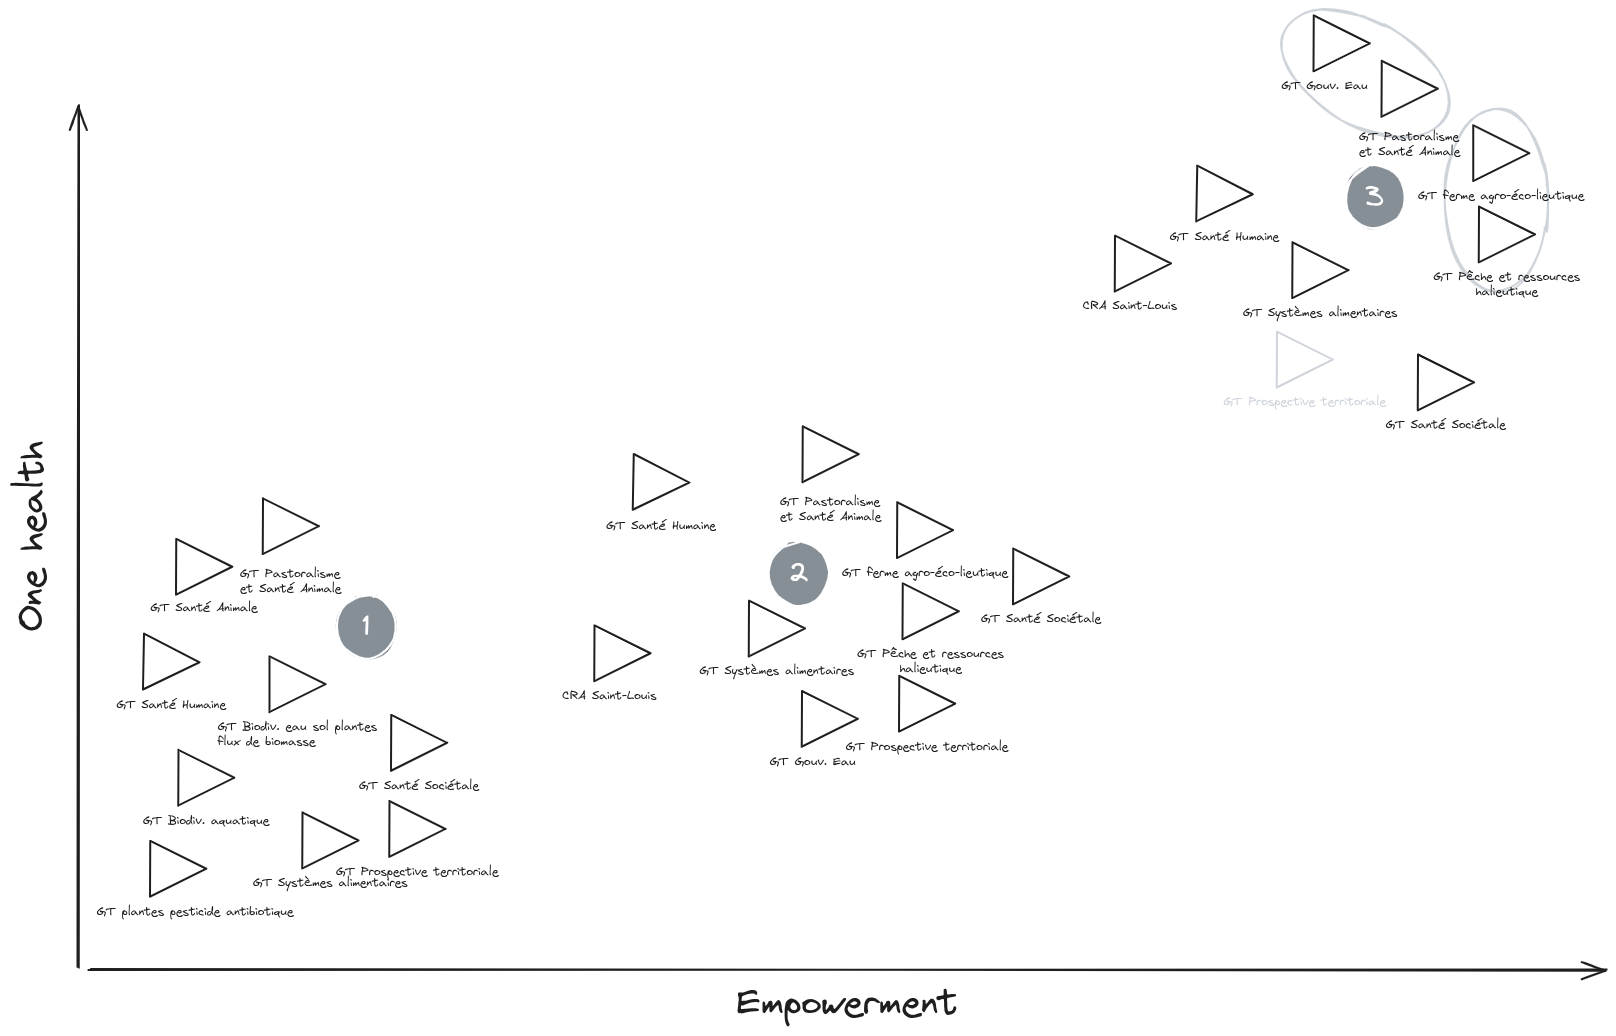
\includegraphics[width=1\linewidth]{img/Drawing 2025-09-07 11.03.30.excalidraw.png}
    \caption{Agencement des différents groupes porté par les scientifiques du projet au travers des 3 phases du projets en fonction de leurs prise en compte de l’objectif On-Heath et de l’émancipation des acteurs. On constate des réarrangement et des convergeances entre les groupes au fur et à mesure de l}
    \label{fig:alignement-proj}
\end{figure}

Au fil des trois phases que nous avons identifiées — éléments disjoints, premiers rapprochements, puis agencement en acte —, le cadre par les agencements permet de lire moins une << progression linéaire >> qu’une succession de reconfigurations où humains, non-humains, règles et dispositifs se couplent différemment. D'abord dans des reconfiguration dans les groupe thématiques, puis une fois ces groupes maturé, entre groupe thématique (c.f. fig. \ref{fig:alignement-proj}).

Dans la veine des travaux qui conçoivent l’agencement comme une composition socio-écologique et matérielle \parencite{hertz_knowledge_2025}, nos observations montrent que l’alignement ne procède pas seulement d’un rapprochement de représentations, mais d’un travail patient sur les prises et attaches qui rendent certaines connexions tenables : un protocole de suivi, un bassin de pisciculture, un collectif d’éleveurs, une contrainte hydrique, un calendrier agricole. Chaque phase correspond alors à un état transitoire des agencements : d’abord dispersés et concurrents, puis stabilisés par quelques médiations partagées, enfin performés sur le terrain par des dispositifs concrets (parcelles fourragères, pisciculture, ateliers ComMod) qui font tenir ensemble des mondes auparavant disjoints.

Cette lecture gagne en intelligibilité si l’on réinscrit les << moments constitutionnels >> affectifs dans la grammaire de la traduction mise en évidence par \textcite{callon_techno-economic_1990} dans le célèbre cas des coquilles Saint-Jacques : problématisation, intéressement, enrôlement, mobilisation. Les épisodes marquants (révélation des pollutions chimiques, conflits pêcheurs autochtones/allochtones, désir local d’expérimenter le fourrage) agissent comme des opérateurs d’intéressement : ils resserrent des attachements autour d’objets et de risques tangibles, déplacent des frontières d’intérêt, ouvrent la possibilité d’un enrôlement. Autrement dit, l’affect fonctionne comme un mécanisme de verrouillage, d'encrage relationnel (on s’engage parce que l’on se sent exposé, concerné, relié) qui participe de la réalité et de la réalisation des actions. À l’inverse, lorsque l’affect fait défaut -- participation de pure conformité, indicateurs sans adresse, prospective trop distante --, l’intéressement reste fragile et l’agencement se délite, à l’image des tentatives avortées que décrit Callon lorsque les acteurs ne reconnaissent plus la << bonne >> porte d’entrée dans le problème.

Enfin, replacer nos résultats dans l’inspiration de \textcite{hertz_knowledge_2025} revient à souligner le caractère sensible des agencements : ce sont des architectures où flux de matière et d’information (eau, biomasse, données), institutions (règles de pêche, procédures sanitaires), et artefacts (jeux sérieux, bio-banques, bassins) co-évoluent, influencés et influançants les affectes. Le passage de la phase 2 à la phase 3 n’est pas seulement narratif ; il correspond à une capacité accrue de circularité (des savoirs, des nutriments, des revenus des agriculteurs ou des pêcheurs qui influence le bien vivre.) et à un renforcement des liens -- quand un même dispositif (par exemple la pisciculture) devient pivot à la fois pour la nutrition, la régénération halieutique, la gestion des connflits entre pêcheurs et la gestion hydrique. C’est précisément là que l’affect participe de l’agencement : les dispositifs qui font sentir des bénéfices et des vulnérabilités partagés sont ceux qui tiennent et reconfigurent durablement les alliances. Cette articulation explique pourquoi certaines convergences observées (pastoralisme–agroécologie, pêche–ferme agrécolieutique) se renforcent, quand d’autres (étiquetées << One Health >> mais faiblement outillées) sont restées au stade déclaratif.


\subsection{La participation comme mot d’ordre pluriel et controversé}

La participation apparaît dans les documents du projet comme un mot d’ordre consensuel : chacun la revendique, mais sans toujours désigner la même chose. Cette polysémie n’est pas nouvelle ; \textcite{arnstein_ladder_1969}, montrait déjà que l’appel à << impliquer >> peut recouvrir des positions très différentes allant de la manipulation symbolique à la véritable délégation de pouvoir. Dans notre cas, nous retrouvons cette diversité : participation réduite à la consultation dans certains groupes (ex. collecte de données biomédicales), participation pédagogique dans d’autres (formations vétérinaires), et participation délibérative plus avancée dans les démarches de co-modélisation. L’unanimité affichée masque donc une pluralité de régimes de participation, dont les effets concrets sur l’alignement diffèrent fortement.

Dans cette perspective, la posture adoptée dans les démarches de modélisation d’accompagnement (ComMod) \parencite{barreteau_our_2003, barreteau_framework_2010}  occupe une place singulière. Là où la participation peut parfois se limiter à une validation d’options déjà cadrées, ComMod repose sur une mise en discussion des représentations elles-mêmes, via des jeux de rôles, scénarios ou modèles co-construits. La participation ne consiste plus seulement à << apporter une voix >> mais à transformer collectivement les cadres de pensée et d’action \parencite{etienne_modepour_2010}. Cette ouverture méthodologique confère à la participation une puissance de stabilisation (en alignant des visions divergentes autour de règles partagées) et une capacité d’émancipation (en permettant aux acteurs locaux de reformuler les problèmes et d’imaginer des solutions qui leur appartiennent).

Il est frappant de constater que lorsque les facilitateurs ComMod tiennent cette posture -- ni experts prescripteurs, ni simples observateurs --, les acteurs trouvent un véritable espace d’autonomie. Comme dans le cas des pêcheurs de Mbane, qui confrontés à la disparition de la biomasse halieutique, blamaient les pêcheurs maliens travaillant sur zone. Ce << lâcher-prise >> des chercheurs permet aux participants d’expérimenter de nouvelles règles, de tester des compromis, d’inscrire leur expérience dans la fabrique du commun. Là où la participation instrumentale tend à renforcer la dépendance envers les experts, la participation telle qu’opérationnalisée dans ComMod ouvre un chemin d’auto-organisation et de capacité d’agir. C’est précisément dans cette tension entre contrôle et émancipation que se joue la portée transformative de la participation : non pas un mot d’ordre consensuel, mais un champ de pratiques où les modalités d’engagement déterminent la robustesse et la durabilité des agencements collectifs.

\subsection{Les moments affectifs comme déclencheurs de reconfigurations}

Les dynamiques observées dans les Living Labs sénégalais montrent que l’alignement entre groupes thématiques n’émerge pas uniquement de débats rationnels ou de cadrages institutionnels. Ce sont souvent des moments marqués par une intensité affective — un choc, une dispute, une révélation — qui déclenchent des reconfigurations. La mise en évidence de pollutions chimiques invisibles dans l’eau du lac~\parencite{}, les tensions entre pêcheurs autochtones et allochtones ou encore l’enthousiasme collectif autour de l’expérimentation de cultures fourragères ont agi comme des révélateurs. Ces épisodes fonctionnent comme des « moments constitutionnels » au sens de Jasanoff : ils fragilisent les cadres habituels et ouvrent un espace de redéfinition des priorités. Autrement dit, c’est lorsque les connaissances se traduisent en expériences vécues, sensibles, que les alliances se transforment réellement, font sens, et dessinent les réelles contributions aux problématiques territoriales.

Cette dimension rejoint les propositions récentes autour du « savoir affectif » (\textit{affective knowing}, dans \textcite{hertz_knowledge_2025}) : un savoir qui ne vaut pas seulement par son contenu cognitif mais par sa capacité à être ressenti et à mobiliser les acteurs. Dans notre cas, l’affect a joué un rôle de catalyseur pour l’intéressement, au sens de \textcite{callon_techno-economic_1990}, en rendant certains problèmes concrets et pressants. Là où les indicateurs ou protocoles restaient abstraits, l’expérience partagée d’une vulnérabilité -- boire une eau contaminée par des substances chimiques, perdre des revenus de pêche, voir ses troupeaux menacés -- a rendu possible un enrôlement durable des acteurs. Le passage d’un savoir distant à une expérience située transforme la discussion en engagement, et l’information en action collective.

L’effet de ces moments affectifs dépasse cependant l’instant. Ils contribuent à renforcer la robustesse des agencements en inscrivant une dimension émotionnelle et mémorielle dans les alliances. En ce sens, l’affect n’est pas un élément accessoire mais un opérateur central de stabilisation : il donne chair aux dispositifs et nourrit un sentiment d’appartenance. En même temps, il comporte une part d’imprévisibilité, car les affects peuvent aussi raviver des clivages ou exacerber des conflits. C’est pourquoi l’accompagnement méthodologique — et notamment la posture des facilitateurs ComMod -- est crucial : il s’agit de transformer ces intensités en ressources pour l’action collective, plutôt que de les laisser se dissiper ou se rigidifier. Les moments affectifs apparaissent ainsi comme des fenêtres d’opportunité, à partir desquelles des imaginaires concurrents peuvent être négociés et des pratiques recomposées.

\subsection{Entre sectorialisation et intégration : la difficile opérationnalisation du One Health}

Le projet Santés \& Territoires illustre bien les limites d’un usage trop générique du terme One Health. Dans sa formulation internationale, le concept se veut intégrateur — réunissant santé humaine, animale et environnementale -- mais il reste souvent une bannière normative, invoquée plus qu’incarnée. Dans les pratiques des groupes thématiques, One Health n’a réellement pris sens que lorsqu’il a été situé : par exemple, lorsqu’il s’est matérialisé dans les parcelles fourragères qui relient besoins pastoraux, fertilité des sols et nutrition humaine, ou dans la pisciculture qui articule biodiversité, revenus alimentaires et gouvernance de l’eau. Autrement dit, l’intégration One Health ne devient opératoire que dans des configurations concrètes, délimitées, qui engagent directement les acteurs.

Cette nécessité de situer One Health renvoie au « décalage prométhéen » dont parle \textcite{anders_obsolescence_1956} : le fossé entre la puissance de nos concepts ou technologies et la capacité des individus à s’y reconnaître et à les traduire dans leurs vies. Tant que One Health demeure une idée abstraite portée par des institutions internationales, il reste hors de portée des communautés locales. Lorsque ce décalage se réduit -- c’est-à-dire lorsque le concept touche à des préoccupations vitales, ressenties et partagées --, il devient moteur d’action. C’est précisément ce que nous avons observé : le passage de One Health comme slogan à One Health comme expérience s’est joué dans l’articulation avec des enjeux concrets dans les living labs du Lac de Guiers.

La réduction de ce décalage est rendue possible par les processus d’alignement entre groupes et par les dispositifs qui donnent une consistance affective et matérielle au concept. Les alignements ne dissolvent pas les divergences sectorielles (biomédical, agronomique, socio-écologique), mais sont des points de jonction où les perspectives se rejoingnent pour devenir tangibles et opératoires. Le One Health doit être encré dans des situations d'actions (territoires, acteurs, problématiques) qui oriente les changements de pratiques. Il doit servir de bousole pour tendre vers l'amélioration des santés. En ce sens, l’opérationnalisation du One Health est moins une affaire de définition qu’une affaire de mise en situation, où les acteurs peuvent reconnaître leur place et agir collectivement.

\subsection{La place des chercheurs : entre facilitation, médiation et portage d’agenda}

L’expérience du projet Santés \& Territoires invite à réinterroger la place des chercheurs dans les dispositifs participatifs. Contrairement à l’idéal d’extériorité souvent revendiqué par les sciences sociales ou environnementales, les chercheurs ne peuvent pas se tenir en surplomb. Ils sont engagés dans les dynamiques qu’ils observent et contribuent à les façonner, qu’ils le veuillent ou non. La littérature souligne régulièrement cette tension : pour \textcite{laslaz_jalons_2017}, une posture de retrait réflexif est encore possible, mais nos activitées dans le projet montrent que dans le cadre des Living-Labs, une telle position apparaît intenable. Les chercheurs sont sollicités comme facilitateurs, médiateurs, parfois même comme garants institutionnels. Leur rôle déborde nécessairement celui de simples producteurs de savoir.

Pour autant, cet engagement ne se traduit pas par une position stabilisée ou « idéale » à occuper. Nos observations renvoient plutôt à une forme de navigation négative \parencite{morizot_manieres_2020}: les chercheurs progressent en identifiant les rôles qu’ils ne veulent pas assumer — celui d’expert prescripteur qui impose des solutions, celui d’animateur neutre qui se contente de distribuer la parole, ou encore celui d’acteur institutionnel qui verrouille les compromis. Ce processus d’évitement, loin de signifier un désengagement, constitue au contraire une manière de préserver des espaces d’autonomie pour les autres participants. La posture des chercheurs se construit donc par retraits successifs, par refus d’occuper certaines places, ce qui laisse émerger des configurations plus ouvertes et négociées.

Cet engagement ambivalent soulève une question éthique et politique forte : jusqu’où les chercheurs doivent-ils s’impliquer dans la transformation qu’ils accompagnent ? L’équilibre est fragile entre la tentation d’imprimer une orientation (au risque d’imposer un agenda) et le désir de se retirer (au risque de laisser se reproduire des rapports de pouvoir existants). La valeur ajoutée de l'approche ComMod tient précisément dans cette tension : les chercheurs ne dictent pas les solutions, mais ils créent les conditions pour que les acteurs puissent s’émanciper et expérimenter. Leur engagement consiste moins à trouver une juste place une fois pour toutes qu’à assumer une posture mobile, réflexive et négative, où l’art de la facilitation s’apprend dans le refus de certaines évidences.

\subsection{Temporalités et échelles d’action : entre prospective et urgences locales}

Les Living Labs du projet Santés \& Territoires révèlent un écart important entre des temporalités hétérogènes : celle des chercheurs et des institutions, rythmée par des projets pluriannuels et des horizons prospectifs (2027 pour santés \& Territoires), et celle des populations locales, centrée sur les urgences quotidiennes liées à la subsistance, à l’eau, aux troupeaux ou aux captures de pêche. Comme l’a montré \textcite{fassin_raison_2010}, le rapport au temps est indissociable d’un rapport moral : les interventions humanitaires -- et, peut être par extension, les interventions scientifiques quand elles ont l'impression de dévoiler une crise -- se situent dans une tension permanente entre urgence (soulager ici et maintenant) et avenir (transformer durablement). Dans notre cas, les démarches prospectives portées par les chercheurs apparaissent souvent trop lointaines pour les acteurs locaux, tandis que les réponses aux urgences semblent dérisoires au regard de l’ambition systémique affichée.

Cette tension temporelle peut aussi être lue à travers la réactivation par \textcite{fassin_science_2009} de la métaphore de Walzer : certains scientifiques restent « dans la caverne », immergés dans l’action et ses contradictions, tandis que d’autres cherchent à conserver une position de surplomb de la caverne, prétendant voir la scène dans son ensemble. Le projet Santés \& Territoires illustre l’ambivalence de ces postures. Les chercheurs impliqués dans les ateliers participatifs vivent les conflits et les affects au même rythme que les communautés locales, mais d’autres acteurs académiques ou institutionnels, à distance, cadrent le projet à partir d’horizons temporels éloignés (prospective 2040, scénarios globaux One Health). Si pour les chercheurs du projet, il serait idéal d'arriver à se tenir au seuil de la caverne, ni trop loin pour ne pas proposer des solutions hors sol, dans une posture critique qui empêche d'avancer, ni complètement dedans pour ne pas perdre de vue le théâtre des opérations. L’articulation entre ces postures est délicate : trop d’immersion fait perdre la vue d’ensemble, trop de surplomb éloigne des réalités vécues.

Enfin, la critique de la temporalité de l’aménagement formulée par \textcite{virilio_fin_2023} éclaire aussi notre matériau. Pour lui, la vitesse moderne tend à écraser le temps long et à privilégier l’instantané, au risque de désarticuler les processus de transformation. Dans les Living Labs, cette critique prend corps : la logique des projets financés par bailleurs impose un calendrier rapide, des délivrable pour pouvoir "décaisser", orienté vers des livrables, alors que les alignements observés entre acteurs se construisent sur un temps beaucoup plus lent, fait d’épreuves, d’affects et d’expérimentations. La vitesse institutionnelle et financière entre ainsi en contradiction avec la temporalité relationnelle et écologique nécessaire à l’opérationnalisation de One Health. C’est dans la capacité à négocier ces régimes temporels discordants -- urgence, lenteur, prospective -- que se joue la durabilité des agencements construits.

\subsection{Vers une transformation systémique : enseignements du cas sénégalais}

L’un des résultats saillants du projet Santés \& Territoires est que tous les acteurs engagés dans le processus ont bénéficié, à des degrés divers, d’une forme d’aspiration collective. Chercheurs, techniciens, élus, agriculteurs ou éleveurs ont trouvé dans l’expérience des Living Labs un espace pour élargir leurs horizons et se confronter à d’autres manières de penser et d’agir. Même si cette dynamique n’a pas toujours produit un alignement parfait, elle a permis un apprentissage mutuel : les chercheurs biomédicaux se sont familiarisés avec les enjeux agroécologiques, les praticiens agricoles ont découvert les logiques sanitaires, et les acteurs locaux ont acquis des repères sur la complexité du concept de One Health. Autrement dit, le processus a généré un capital cognitif partagé, qui constitue une première condition pour envisager des transformations systémiques.

Cependant, cette montée en compétence collective se heurte à des difficultés persistantes lorsqu’il s’agit de traduire l’appropriation des concepts en véritable émancipation. Les populations locales, dans les deux Living Labs, se sont saisies des outils participatifs pour formuler leurs propres priorités et tenter de  négocier des solutions adaptées. Pourtant, du côté de certaines institutions de recherche, l’abandon du contrôle des agendas scientifiques reste plus problématique. Laisser de la place aux acteurs non académiques, accepter que leurs savoirs redéfinissent les questions de recherche, demeure un exercice délicat. Ces réticences traduisent une tension structurelle : la volonté de promouvoir une science en société transdisciplinaire et participative, tout en maintenant les logiques de légitimation académique et de productivisme scientifique.

Ce constat invite à relativiser la portée du modèle. Le cas sénégalais montre que la transformation systémique n’est pas seulement une affaire d’outils ou de méthodologies, mais de rapports de pouvoir, d'affects et de reconnaissance. Le partage du langage autour One Health a indéniablement favorisé des rapprochements et donné un vocabulaire commun, mais son efficacité repose sur la capacité des institutions à accepter une redistribution des rôles. Si les chercheurs demeurent trop enclins à cadrer les trajectoires, l’émancipation des participants locaux restera partielle. À l’inverse, chaque fois qu’un espace de négociation ouvert est rendu possible -- comme dans les expérimentations fourragères ou piscicoles --, les alignements produisent des effets tangibles et durables. C’est sans doute là l’enseignement le plus fort : pour que les Living Labs deviennent de véritables moteurs de transformation systémique, il ne suffit pas d’aligner des représentations, il faut aussi redistribuer les capacités d’agir pour gagner en liberté \parencite{sen_development_1999}.

\section{Conclusion}

L’étude du projet Santés \& Territoires au Sénégal met en lumière un processus d’alignement progressif, marqué par des phases de dispersion initiale, de rapprochements incertains puis d’agencements stabilisés. Ce cheminement, non linéraire, s’est nourri de rencontres, de tensions, de conflits parfois, mais aussi d’expériences affectives partagées qui ont ouvert des possibles (disparitions des poissons, présence de produits chimique dans l'eau). Cette dynamique confirme la fécondité de l’approche par les agencements pour analyser les projets de transformation dans leur dimension relationnelle et située. Elle permet de comprendre comment des éléments hétérogènes -- humains et non humains, savoirs scientifiques et pratiques locales, institutions et affects -- parviennent à se coordonner dans des configurations qui rendent l’action possible.

Relue à travers la grille proposée par \textcite{anders_obsolescence_1956}, cette analyse prend une portée philosophique supplémentaire. Anders soulignait le « décalage prométhéen » entre la puissance de nos concepts ou technologies et la capacité des individus à s’y reconnaître et à les traduire dans leur vie. Nos résultats suggèrent que la lecture par agencements et la sociologie de la traduction offrent une manière concrète de réduire ce décalage : en situant les concepts globaux comme One Health dans des dispositifs matériels et affectifs locaux, ils facilitent le passage à l’action transformatrice. Loin de rester des slogans ou des promesses, ces notions deviennent opératoires dès lors qu’elles s’incarnent dans des pratiques situées et qu’elles mobilisent les acteurs par l’expérience vécue. Dans le processus, les participants gagnent en capacité d'action et donc en liberté au travers des expérimentations, et de leurs constructions
\parencite{sen_development_1999}.

Enfin, cette étude confirme l’importance de la co-construction des imaginaires. Comme le rappellent \textcite{castoriadis_domaines_1999,beckert_uncertain_2018}, dans un monde d’incertitude radicale, ce sont les récits, modèles et fictions collectivement partagés qui orientent les décisions et coordonnent l’action. Lorsqu’ils sont imposés d’en haut ou portés par quelques acteurs dominants, ces récits risquent d’exclure et de figer les possibles dans des cadres souvent pensé à l'extérieur du système. À l’inverse, les démarches participatives et les dispositifs de modélisation d’accompagnement permettent de produire des modèles avec les parties prenantes, et non pour elles. Ces modèles co-construits façonnent l’avenir de manière plus équitable et plus durable, avec un regard ancré par les penseurs du territoire, en redistribuant les capacités d’imaginer, de dire et d’agir. En ce sens, l’expérience sénégalaise n’est pas seulement un cas local : elle éclaire les conditions par lesquelles des projets transdisciplinaires peuvent devenir de véritables laboratoires de transformation systémique, là où se rencontrent savoirs, affects et engagements partagés.


\printbibliography

\end{document}